

\begin{frame}{Manchester encoding}
\begin{tikzpicture}
\node (fig) { 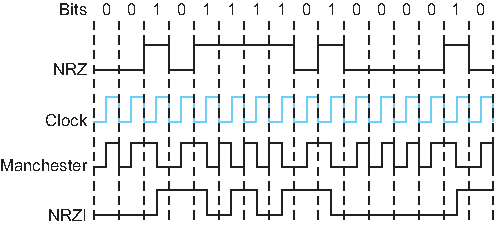
\includegraphics[width=0.9\textwidth]{../physical/SysApproach-2-Fig-25.pdf} };
\end{tikzpicture}
\imagecredit{Figure 25 from Section 2.2 of \textit{Computer Networks: A Systems Approach} (6th ed) (Peterson and Davie)}
\end{frame}

\begin{frame}{problem with Manchester}
    \begin{itemize}
    \item fixed the problem of too few transitions
    \vspace{.5cm}
    \item but now most transitions don't send information
    \item means we aren't making good use of wire/etc. capacity
    \vspace{.5cm}
    \item there are more clever compromises
        \begin{itemize}
        \item (example: 4B5B encoding)
        \end{itemize}
    \end{itemize}
\end{frame}
